% status: 0
% chapter: TBD

\title{Twitter sentiment analysis of the Affordable Care Act in 2018}


\author{Michael Smith}
\affiliation{%
  \institution{Indiana University}
  \streetaddress{School of Informatics and Computing}
  \city{Bloomington} 
  \state{Indiana} 
  \postcode{47408}
  }
  
\email{mls35@iu.edu}



\renewcommand{\shortauthors}{M. Smith}


\begin{abstract}
The mission of this project is to utilize technologies and cloud
computing to perform a successful sentiment analysis through software
deployment written in python.  The project encompasses social media
mining of twitter, analysis of data through apache spark, and testing
on a multimachine cluster.  Benchmarks on the cloud infrastructure
Digital Ocean was performed in 1 to 3 node clusters and various
machine specifications were tested.  The main spark program was a
python script which processed over 15000 tweets associated with the
affordable care act.  Each tweet was processed through natural
language processing techniques and its negative or positive sentiment
was identified.  Visualizations of the processed data were produced to
show outcomes.  An automated deployment of this analysis was produced
through the configuration tool ansible.

\end{abstract}



\keywords{hid-sp18-707, Apache Spark, Sentiment Analysis, Ansible, Python}



\maketitle

\section{Introduction}

The current political climate of the United States is divided on many
important issues.  There is a disconnect between the motivations of
the politicians of today and what is deemed important to the American
people.  The affordable care act (ACA) also known as Obamacare has
been a target of the GOP, however it is uncertain if that sentiment is
shared by most Americans.  With a law that affects millions of
Americans it is often difficult to gauge how the American people feel
about the current health care law.  It is the goal of the project
utilize big data technologies to gauge how Obamacare is viewed through
social media.

\section{Project Overview}

The project is designated into four phases as seen in
figure~\ref{f:overview}.  Interface with twitter to acquire data for
future analysis, the goal of this to accumulate a substantial number
of tweets that provide affordable care act sentiment.  The second
phase involves the development of an ansible playbook that will setup
a three node cluster of virtual machines with all the environment
components necessary to deploy spark, fetch files, and run python
scripts all in an automated process.  The third phase in the project
entails development of a spark program that will run successfully on a
cluster and analyze the twitter data which will provide an overview of
the sentiment.  The final phase involves testing the deployment on a
cloud infrastructure with single and three node benchmarks, various
node specifications such as the amount of cores and allocated memory
will also be benchmarked.

\begin{figure}[!ht]
  \centering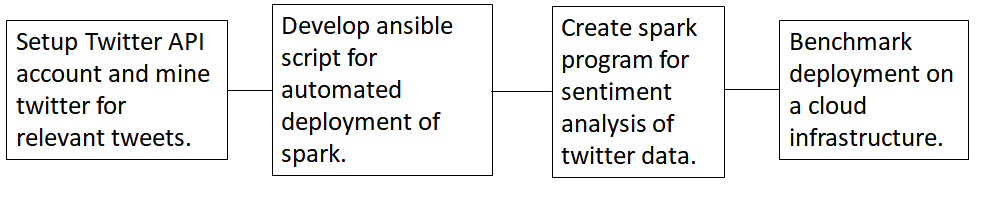
\includegraphics[width=\columnwidth]
  {../../hid-sp18-707/images/overview.png} \caption{Project Overview}
\label{f:overview}
\end{figure}

\section{DigitalOcean}

The benchmarking the deployment on a cloud infrastructure is one of the
primary objectives in this project.  The cloud service DigitalOcean,
Inc was utilized for software deployment.  While they are an American
company, they possess datacenters in New York, San Francisco,
Amsterdam, Singapore, London, Frankfurt, Toronto and Bangalore.  They
offer a range of virtual machines with RAM allocation from 1 to 192
GB, vCPU from 1 to 32 cores, and SSD storage from 25 GB to 3840 GB.
Their service allows the resizing of existing virtual machines to
different specifications allowing ease in comparing performance.  For
all virtual machines the OS ubuntu 16.04.4 was utilized.

\section{Twitter}

The social media platform Twitter is a service utilized by millions of
users who interact through micro-blogging in 280 characters or
less~\cite{www-statista}.  While the messages are brief the breadth of
information available is an ideal resource to perform a sentiment
analysis of a given topic.  Twitter offers an API that allows
developers to establish an account to collect tweets of
interest~\cite{www-twitterapi}.  It is subdivided into two components:
a representational state transfer REST and streaming API.  The REST
component allows the ability to query a twitter users account or
modify an account with extra permissions.  The streaming API delivers
tweets based on selected search terms and will deliver data in real
time.  Data is returned to the user in a JavaScript Object Notation
format or JSON.  Some notable aspects of the JSON schema include user
id, text of the tweet, user location, and timestamp.  The streaming twitter API
was selected to gain real time data regarding the topic of interest.

\subsection{Twitter mining}

In order to acquire unique tweets, a python script was developed using
the twython library which is a python wrapper for the twitter
API~\cite{www-twy}.  The code for this script was adopted from Joel
Grus~\cite{www-fetchtweet}.  The script fetchtweets.py will first
authenticate with twitter through unique consumer keys and access
tokens.  Secondly, will listen for tweets that contain keywords and
capture data objects and store them locally in a JSON format.  The
keywords utilized for selecting tweets contained any of the following
phrases: obamacare, ACA, or various combinations of affordable care
act.  An additional requirement for data aquisition relied on setting
language key value to be english.  The script was triggered to shut
off after 1000 tweets and was repeatedly ran over a period of two
weeks.  Once the dataset contained over 15,000 tweets the data
acquisition phase of the project was concluded.


\section{Automated Deployment}

Deployment of an apache spark program can be a tedious process and
sensitive to potential errors depending on the computing environment
of the user.  This creates a difficult hurdle for collaboration and
repeatability.  In order to automate the setup and create a reliable
application, the technology ansible was utilized for system
configuration~\cite{www-ansibleweb}.

\subsection{Ansible}
Ansible is an open source software used for automated provisioning of
computing environments.  This tool is beneficial in assurance that
each node is setup with the appropriate dependencies and environment
for a consistent execution.  Ansible executes a series of commands
from a file in the YAML format which is referred to as a
playbook~\cite{www-ansible}.  A configuration will be checked to see
if it is already present on the target VM, if not the play will be
installed otherwise the command is skipped.  The YAML format is human
readable and utilizes indentation similar to python.  In order to
successfully run a playbook on a cluster of nodes or a single node.
It is vital that a secure connection be made, most commonly through a
secure shell key also known as an SSH key.  SSH ensures security
between nodes so that configuration is only occurring where it is
allowed, moreover the convenience of a secure connection without a
password.  For the purpose of this project, an ansible playbook was
developed to install all dependencies and programs necessary to
automate a spark cluster configuration.

\subsection{Ansible playbook design}
Deployment on Digital Ocean required a manual input of ip addresses
and username within the groups of either Master or Node section in an
inventory.txt.  The ansible playbook calls the inventory file along
with the main.yml to initiate deployment.  The main features of the
main.yml are detailed in the process of configuration below.

\begin{itemize}

\item \textbf{Python}: In order for ansible to execute its yaml file
 which is written in python, it needs to be installed on the
 target vm.  The command getfacts will receive information about the
 vm including whether or not python has been installed.  If it is not
 present this play will execute an installation of python minimal.

\item \textbf{Variable Assignment}: The ip address of the master node
 is utilized in multiple plays during deployment. To prevent the
 requirement of the user to manually set this value within the
 playbook. All ip addresesses of hosts were gathered and the variable
 ENV was created and assigned only the master ip address through the
 set facts command.
 
\item \textbf{Java}: Apache spark runs on top of Java, thus all nodes
 require its installation.  Selecting the correct Java version is
 important as versions of java below 8 will not run on Spark 2.2.0 or
 higher.  Therefore java 8 was installed which is sufficient for spark
 2.3.0.

\item \textbf{Apt}: Apt packages are then installed including
python-pip for library installations, python-dev, and also python-tk.
A follow up script will then verify that python-pip is upgraded to the
latest version.

\item \textbf{Spark}: Spark 2.3.0 is then downloaded and extracted
using the geturl command.

\item \textbf{Python packages}: Python library installations via
Python-pip added the necessary dependencies for the spark program are
installed including: NumPy, TextBlob, Matplotlib, and WordCloud.

\item \textbf{wget}: The twitter.json dataset and
main.py script is then fetched through wget with ansible shell
commands.  Conditional statements within the shell script will first
verify the presence of files to prevent replicated files, this adds
convenience to repeated playbook runs.

\item \textbf{start-master.sh}: Host specific plays on the master
node begin spark in standalone mode.

\item \textbf{start-slave.sh}: Slaves are then started and allocated the
 proper ip address configurations to connect with the master.

\item \textbf{spark-submit}: The final command in the playbook
 initiates the spark-submit command to run main.py.

\end{itemize}



\section{Apache Spark}

As the size of data has grown far beyond the processing capacity of a
single machine, a need developed to process large data sets in a
timely and efficient manner.  It has become commonplace for data
processing to occur in a cluster computing environment which is
referred to as high performance computing or HPC.  A well known
technology Apache Hadoop written in Java is capable of batch processng
data over a cluster of machines with a programming model known as
MapReduce~\cite{www-hadoop}.  Unfortunately Hadoop possess some
disadvantages such as the inability to perform streaming processing,
it uses only Java for writting applications and processes data in a
disk based manner which leads to a cost performance with big
data~\cite{www-aaspark}.  Apache Spark was created at UC Berkeley AMP
Lab and was created in such a way that helped overcome some of the
shortcomings of Hadoop.  Spark applications can be written in several
languages such as R, Java, Scala, and Python which adds flexibility
for the user to write spark programs in the language of their
choosing.  Instead of disk based processing Spark processes data
in-memory which will make data easier to access and increase overall
speed.  The core functionality in spark lies within the RDD or
resilient distributed dataset.

\subsection{RDD}
An RDD is a collection of objects with unique features that make it
advantageous for big data applications.  They are immutable which
means that when performing a computation on an RDD, it is not modified
but a new RDD is created as the computed output~\cite{www-hpspark}.
RDDs can be split into partitions for distribution amongst a cluster
of machines with different tasks acting on it. RDDs are considered to
be resilient or fault tolerant which affords spark the ability to
reprocess a partition if a worker node fails in the cluster.  There
are two ways that an RDD is acted up which is an action or a
transformation.  Spark is referred to as a lazy evaluator, which means
it will apply a transformation until an action is called.  This
methodology does not waste resources and only does enough to satisfy
the action when called.  When an action is completed nothing is saved,
this can create issues when invoking multiple actions on the same RDD.
In order to increase effiency Spark allows caching of an RDD or allow
it to persist across a cluster in memory or on disk.  All of these
features of RDD enhance the cluster computing functionality of Spark.


\subsection{Spark Architecture}

The main spark program is run in the driver which creates RDDs,
performs necessary actions on the data and initiates a sparkcontext.
The sparkcontext will connect to a cluster manager which can be a
Mesos, YARN, or sparks built-in standalone cluster manager, these will
assist resource management on the cluster~\cite{www-aaspark}.  The
standalone client mode was selected for this project, its driver
program runs on the master node and it will schedule jobs based on a
first in and first out order FIFO. It is the responsibility of the
driver to split the applications into sets of tasks to send to the
cluster manager which will launch executors on worker nodes for
processing.  The processed result is sent back to the driver through
the cluster manager.


\subsection{Core components of Spark}

Spark can be categorized into several primary components that serve
different functions within spark such as Spark Core, Spark SQL, Spark
Streaming, MLlib and GraphX~\cite{www-hpspark}.

\begin{itemize}

 \item\textbf {Spark Core}: Spark core is the primary framework with
 APIs in Scala, Java, Python and R.

 \item\textbf{Spark SQL}: Spark SQL enables the usage of
 SQL queries on data frames within a spark program. 

 \item\textbf{Spark streaming}: Enables the batch processing through
the utilization of repeatable code through sources such as HDFS, Flume
and even twitter.  While the dataset is from twitter, spark streaming
is not utilized for this project so that accurate controlled bench
marking on varied cluster allocations can occur.

\item\textbf{MLlib}: MLlib is a
library enabling the application of various machine learning
algorithms on a dataset for training and testing.

\item\textbf{GraphX}: A library
for graph computation.  The latest version of Spark (version 2.3.0)
was utilized for deployment across all nodes.
\item\textbf{SparkR}: SparkR provides a frontend for R to interface with Spark.

\end{itemize}

\section{Technologies}

Spark and ansible are the two primary technologies utilized in this
project but other technologies were use for specific uses throughout
the project such as python and several libraries and modules described below.

\subsection{Python}
Python is an object oriented programming language, it is considered a
high level programming language because it has to be processed by an
interpreter prior to running~\cite{www-python}.  It is more human
readable than other programming languages and is a valuable tool for
processing data.  Writing in python can be ran in an interactive mode
useful for testing code or and an entire python file can be processed
at once in script mode.  The core python script of this project
main.py was ran on the spark cluster.

\subsection{TextBlob}

Textblob is a python library for processing data consisting of
text~\cite{www-textblob}.  In addition to sentiment analysis this
library also has uses in tagging parts of speech, translating languages
and classification through Naiive Bayes and Decision Trees.  The
sentiment analysis functionality of this library will be the primary
tool used for this project.

\subsection{Matplotlib}

Matplotlib is a python library used for data
visualization~\cite{www-matplot}.  It utilizes NumPy to plot 2D arrays
in python, it offers numerous options regarding the plot type, use of
color, and other functionalities.

\subsection{Numpy}

Numpy is a python library for applying mathematical functions on top
of arrays of varying dimensions~\cite{www-numpy}.  It is more
efficient in processing data than pythons standard list feature making
it superior option for handling larger datasets.

\subsection{Wordcloud}

Wordcloud is a python library created by Andreas Mueller that produces
interesting visualizations of data from a text
file~\cite{www-amueller}.  All words are extracted from a document and
given weight based on the number of occurrences of the word.  The
project image then precomputes the number of places for rectangles in
the image and randomly samples words for placement.  Bigger words will
stand out more due to their high frequency leading to interesting
insights into the text data.

\subsection{Re}

The regular expression module for python allows processing strings by
locating unique sequence of characters in order to add, modify or
delete the string.  This tool facilitates modifying strings at scale
in an efficient manner.

\section{Spark program design}

In order to process the twitter.json dataset the main.py invoked a
number steps with some key functionalities.  Spark allows user defined
functions UDF to develop custom actions on RDDs which was utilized in
this program.  A number of UDF's were generated in order to
effectively process RDDs with the integration of python libraries.
The UDFs process the data by converting all text data from unicode to
ascii.  This prevents future errors when writing the various outputs
to textfiles.  Another UDF encompassed processing text with regular
expression which removes all usernames, hashtags and hyperlinks of
tweets.  Finally leveraging textblob within a UDF allowed the
sentiment analysis of the cleaned tweet and generates a spark
dataframe containing the cleaned tweet with its corresponding
polarity, this was collected and written to an output file called
twittersentimentlist.txt.  Development of the wordcloud afforded some
unexpected issues when dealing with twitter data.  A significant
amount of tweets in the dataset were from retweets which inflated the
weighting of word frequencys in those tweets.  To overcome this
hurdle, all retweeted text could be filtered by utilizing the distinct
operation in Spark.  This removes all text that is identical and will
filter it down to simply one instance of a given retweet.  This RDD
was collected into a text file and passed to the Wordcloud function to
generate an image which is saved as acatextcloud.png.  The final
analysis involved plotting a histogram of all polarity values that
were calculated, those values were selected and stored written to a
list and text file called polaritylist.txt.  The list was plotted with
matplotlibs histogram function to give insight into the twitter
sentiment, the plot was saved as polarityhistogram.txt.  An
overview.txt file was also generated which gives a breakdown of the
number of tweets, retweets, the most popular tweet, and a mean of all
calculated polarities in the dataset.




\section{Results}

What occurred in the spark program is referred to as natural language
processing (NLP) which is defined in the simplest of terms as enabling
a computer to gain meaning from human language.  This can be used in a
number of different ways including sentiment analysis.  The polarity
scoring in sentiment analysis is on a range from -1 to +1 which is a
negative to a postiive sentiment respectively.  Observing the final
output of the distribution of scores found in the histogram in
Figure~\ref{f:polaritytweet}, it is clear that sentiment regarding ACA
is not as negative as Washington makes it out to be.

\begin{figure}[!ht]
  \centering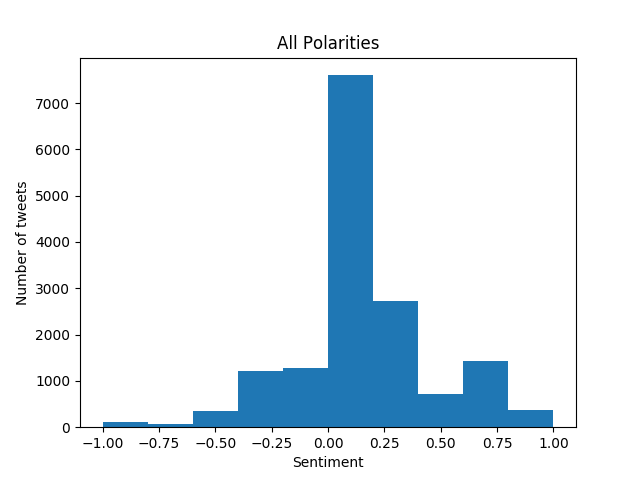
\includegraphics[width=\columnwidth]
  {../../hid-sp18-707/images/polarityhistogram.png}
  \caption{Result of sentiment analysis of all tweets.}
\label{f:polaritytweet}
\end{figure}

While the distribution sentiment is seen to reach both ends of the
spectrum, the majority of sentiment lies predominantly in the slightly
positive range.  When calculating the average sentiment value of all
polarities a value of 0.13 was observed showing consistency with the
histogram visualization.

\section{Worldcloud}
Here is a word cloud at Figure~\ref{f:textcloud}
\begin{figure}[!ht]
  \centering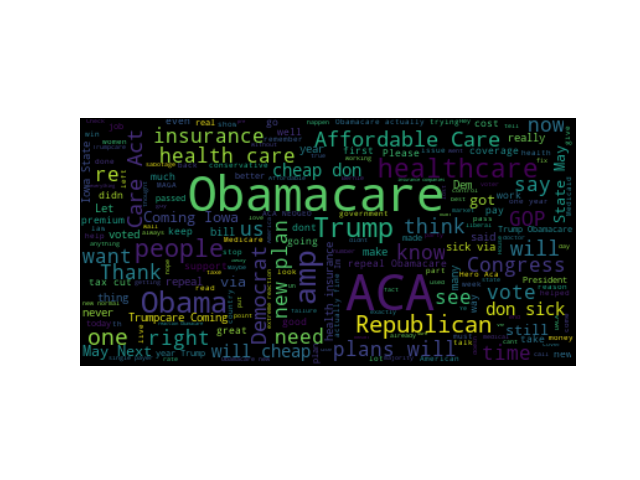
\includegraphics[width=\columnwidth]
  {../../hid-sp18-707/images/acatextcloud.png}
  \caption{Wordcloud
  output of Analysis.}\label{f:textcloud}
\end{figure}





\section{Benchmarks}

The program was tested on 1 node and 3 node clusters through
DigitalOcean service.  The programmed was clocked using pythons time
library to accurately assess completion time.  In addition to
different nodes, the flavor of the nodes was modified to see how
improved computing would affect benchmarks.  Three variants of each
node was assessed with the following specs, Table~\ref{t:my-label}
outlines the different flavors tested, CPU was tested on 1, 2, and 4
vCPUs with an increased memory of 1, 2 and 4 GB respectively.  Each
configuration was tested five times and the average was reported.
The single node cluster saw benchmark average times of 90.18, 71.19,
and 29.75 seconds on the small, medium and high flavors respectively
shown in Figure~\ref{f:singlenode}.
\begin{figure}[!ht]
  \centering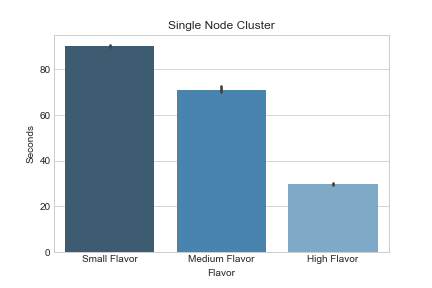
\includegraphics[width=\columnwidth]
  {../../hid-sp18-707/images/singlenode.png}
  \caption{Benchmarks of all flavors on a single node cluster.}
\label{f:singlenode}
\end{figure}

The three node custer had average times of 489.77, 277.86 and 210.05
seconds on small, medium and high flavors as seen in
Figure~\ref{f:threenode}.  The relatively small size of the dataset
~112 Mb will not see a benefit in performance moving to a cluster
which explains why the benchmarks decreased in efficiency when moving
to three nodes.  The limiting factor in speed became the network
between nodes.  In order to limit this effect, all nodes where setup
on the same datacenter located in New York, however a decrease in
performance was still apparent.



\begin{figure}[!ht]
  \centering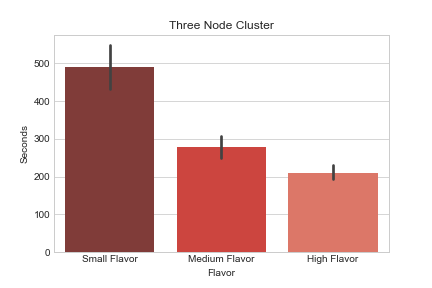
\includegraphics[width=\columnwidth]
  {../../hid-sp18-707/images/threenode.png}
  \caption{Benchmarks
  of all flavors on a three node cluster.}\label{f:threenode}
\end{figure}



\begin{table}[htb]
\centering
\caption{Specification of each flavor tested}
\label{t:my-label}
\begin{tabular}{llll}
Specifications & Small Flavor & Medium Flavor & High Flavor \\
vCPU           & 1 Core       & 2 Cores       & 4 Cores     \\
RAM            & 1 GB         & 2 GB          & 4 GB       
\end{tabular}
\end{table}

\section{Conclusion}

Thie project details a successful deployment of apache spark on a
cloud infrastructure.  The deployment was automated with ansible
configuration management tool.  A spark program was designed that can
process tweets orginally fetched through the Twitter API.  Through
natural language processing the textual data was cleaned and
polarities were calculated for over 15,000 tweets.  The polarities
were visualized in a histogram and a wordcloud to gain insight into
public impressions.  A general sentiment of the affordable care act
was gained from the results showing a distribution of sentiment that
was net positive.  The program was benchmarked in single and three
node clusters with multiple flavor specifications in the digital ocean
infrastructure.  While improved flavors improved benchmarks, single
node performance proved to be superior to the three node counterpart.
A likely reason for this lies in the fact that the small size of the
dataset was sufficiently ran in a single node cluster.  Some
limitations in this methodology is the reliance on the accuracy of
textblob.  Sample size is also relatively small, taking a snippet of
tweets from a two week period in 2018 is not enough to capture
sentiment in an effective manner.  Mining over longer periods of time
would give better insights as sentiments are subject to change over
time.  For future work, it would be beneficial for optimization of
code in the spark program to improve cluster performance and
development of a spark streaming component for real-time processing of
tweets.  Moreover testing sentiment with machine learning
algorithms and benchmarking accuracy against textblob would be a goal for
future work.

\section{Author Biographies}

Michael Smith is a senior quality control analytical chemist at
Creosalus Inc in Louisville, Kentucky.  Michael possesses a MS in
pharmaceutical sciences and a BS in Biology from the University of
Kentucky.  He will obtain his MS in Data Science program from Indiana
University in May 2018.  His current interests are python programming,
data analytics, and spending time with his wife and children.

\begin{acks}

  The author would like to thank Dr.~Gregor~von~Laszewski for his
  support and suggestions to write this paper.  Thank you to all of
  the Teaching Assistants who promptly answered my questions.  Having
  little experience in programming and even less working in the linux
  environment made this course a very challenging but equally
  rewarding experience.

\end{acks}

\bibliographystyle{ACM-Reference-Format}
\bibliography{report} 

